% =============================================================================
% P3 --- version sencilla: criterio de presencia por numero medio de rafagas.
% Sustituye integramente la seccion P3.
% Figura: presencia_media_rafagas.png  (scripts/presencia_media_simple.py)
% =============================================================================
\section{P3 --- ¿Puede el sistema confirmar operativamente la presencia de un dron?}
\label{sec:bloque_presencia}

\subsection{Planteamiento del experimento}
\label{sec:p3_planteamiento}

El recall de caja del \SI{39}{\percent} del experimento P2 mide cuántas ráfagas individuales detecta el modelo, pero esa no es la pregunta relevante para un sistema de vigilancia. La pregunta operativa es más sencilla: \emph{dada una ventana de \SI{0.1}{\second}, ¿hay un dron o no?}

Para responderla se cuenta cuántas ráfagas de clase \emph{drone} detecta el modelo en cada ventana y se compara ese número con un umbral mínimo~$K$: si la ventana contiene al menos~$K$~ráfagas, se declara que hay un dron. El criterio para fijar~$K$ se apoya en una observación muy directa sobre el número medio de ráfagas por ventana.

\subsection{Resultados}
\label{sec:p3_resultados}

La \cref{fig:presencia_media} compara el número medio de ráfagas \emph{drone} detectadas por ventana en las \num{300}~imágenes con dron y en las \num{300}~de interferencia pura del conjunto de prueba. La diferencia es enorme: una ventana con dron acumula de media \num{117,5}~ráfagas, mientras que una ventana sin dron apenas registra \num{0,2}~ráfagas espurias. Esta separación es consecuencia directa del protocolo FHSS de OcuSync, que salta de canal decenas de veces por cada \SI{0.1}{\second} y deja, por tanto, decenas de ráfagas en cada ventana.

\begin{figure}[htbp]
    \centering
    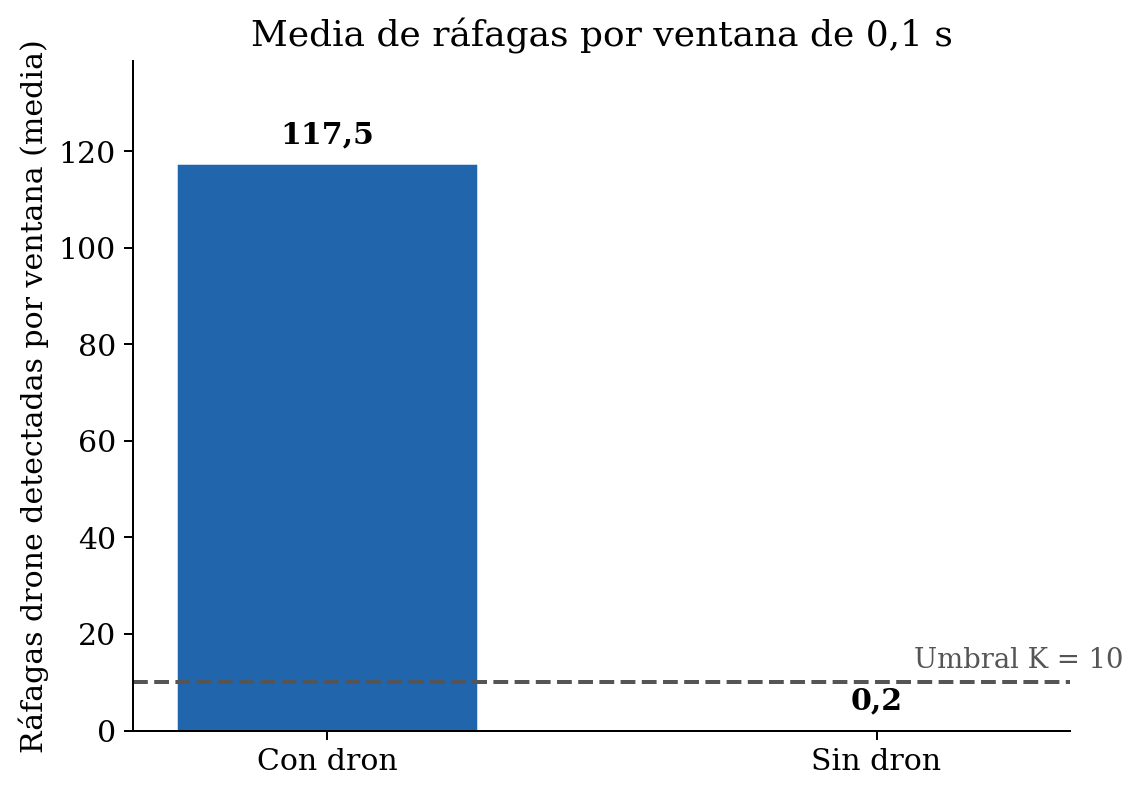
\includegraphics[width=0.65\textwidth]{figuras/resultados/presencia_media_rafagas.png}
    \caption{Número medio de ráfagas \emph{drone} detectadas por ventana de \SI{0.1}{\second}. Las ventanas con dron promedian \num{117,5}~ráfagas; las de interferencia pura, \num{0,2}. La línea discontinua marca el umbral de presencia escogido ($K=10$), situado holgadamente entre ambos niveles.}
    \label{fig:presencia_media}
\end{figure}

Dada esta diferencia, basta con fijar un umbral redondo y conservador. Se elige $K=10$~ráfagas: un valor arbitrario pero seguro, muy por debajo de la media de las ventanas con dron (\num{117,5}) y muy por encima del nivel de ruido de las ventanas sin dron (\num{0,2}). Con este umbral, una ventana se declara positiva solo si el detector encuentra al menos diez ráfagas \emph{drone} en ella.

Aplicado al conjunto de prueba, el criterio $K=10$ clasifica correctamente las \num{600}~imágenes: las \num{300}~ventanas con dron se confirman todas, y ninguna de las \num{300}~ventanas de interferencia produce una falsa alarma. El recall de presencia, la especificidad y la precisión valen \num{1,000}: el sistema no se equivoca ni en un solo caso.

\subsection{Discusión}
\label{sec:p3_discusion}

El resultado de P3 es la confirmación operativa del sistema: aunque el detector falle la mayoría de las ráfagas individuales (recall de caja del \SI{39}{\percent}), la decisión a nivel de ventana es perfecta. La razón es la redundancia del protocolo: con más de cien ráfagas por ventana en una captura con dron, al modelo le sobra con acertar unas pocas para superar el umbral de diez, mientras que en una ventana sin dron no llega a juntarlas nunca. El umbral $K$ actúa así como un filtro que convierte muchas detecciones débiles en una decisión binaria robusta.

La elección de $K=10$ no es crítica: cualquier umbral comprendido entre unas pocas ráfagas y varias decenas produce el mismo resultado sobre el conjunto de prueba, porque las dos poblaciones están muy separadas. Conviene matizar, no obstante, que esta separación se ha medido en el entorno interior controlado del dataset~v3 (\cref{cap:implementacion}); en un despliegue con mayor variedad de distancias e interferencias, el umbral debería recalibrarse observando de nuevo el número medio de ráfagas por ventana en cada clase.
